\chapter{Connaissances biologiques} 

\lettrine{O}{n} s'intéresse dans ce chapitre au manguier et à la cécidomyie des fleurs.
On s'intéresse en particulier à leurs descriptions d'un point de vue biologique, leurs développements et leurs interactions.
Autrement dit, on recense ici les connaissances biologiques nécessaires à la compréhension de notre sujet.


\section{Le manguier}

Le manguier est un arbre qui a un \emph{cycle phénologique} qui lui est propre.
On désigne par cycle phénologique les phénomènes périodiques qui rythment le développement du monde vivant en fonction des variations climatiques saisonnières.
Si l'on observe toujours les mêmes étapes, à savoir une croissance végétative suivie d'une floraison puis d'une fructification et enfin un repos végétatif (avant de recommencer),
il est nécessaire de noter qu'il y a chez le manguier, en sus des conditions climatiques, d'autres facteurs qui influent sur la phénologie tels que la position de l'unité de croissance ou la charge en fruit de l'année précédente \citep{magne2004effet, normand2009axis}.
Il en résulte que le cycle phénologique est très variable d'un manguier à l'autre.
On observe même des différences au niveau d'un même arbre.
Cela implique aussi que le cycle phénologique peut être modifié (dans une certaine mesure) grâce à des opérations techniques, comme la taille par exemple.
Mais il subsiste toujours une phénologie étalée dans le temps à l'échelle d'un verger, on parle alors d'asynchronismes phénologiques.
Quand cet étalement concerne des stades sensibles aux ravageurs, lors de la floraison par exemple, cela implique une disponibilité en ressources assez longue pour les ravageurs, et peut expliquer leur forte présence.

La croissance végétative du manguier est dite rythmique.
Cela signifie que sa croissance est entrecoupée par des périodes de repos.
Durant les périodes de croissance, les branches sont prolongées à leur extrémité par des axes feuillés.
Ces axes sont appelées \emph{unités de croissance}. 
% Si une unité de croissance prolonge la branche dans l'axe, alors elle est dite apicale ; si elle la prolonge sur le côté, elle sera qualifiée de latérale.
Au fil du temps, les unités de croissance perdent leurs feuilles, durcissent et grossissent jusqu'à faire partie intégrante de la branche.
On peut alors voir le manguier comme un empilement d'unités de croissance;
la base du tronc étant l'unité de croissance la plus ancienne et celles qui portent des feuilles les plus récentes \citep{normand2009}.
Des unités de croissance sont visibles sur la figure~\ref{fig:uc}.
\begin{figure}[ht]
 \centering
 \includegraphics[scale = 0.1]{photos/branche.pdf}
 \caption{Photographie d'une branche portant des unités de croissance. Les flèches rouges montrent des unités de croissances. Les flèches bleues montrent les délimitations des unités de croissance antérieures ; la portion de la branche entre deux flèches bleues correspond à une ancienne unité de croissance qui a perdue ses feuilles, grossie et durcie et qui fait désormais partie intégrante de la branche.}
 \label{fig:uc}
\end{figure}


% \begin{wrapfigure}{r}{3.5in}
% %%%%%%%%%%%%%%%%%%%%%%%%%%%%%%%%%%%%%%%%%%%%%%%%%%%%%%%%%%%%%%%%%%%%%%%%%%%%%%%%%%%%%%%
% %%% You will need to add \usepackage{wrapfig} to your preamble to use textwrapping %%%
% %%%%%%%%%%%%%%%%%%%%%%%%%%%%%%%%%%%%%%%%%%%%%%%%%%%%%%%%%%%%%%%%%%%%%%%%%%%%%%%%%%%%%%%
%  \centering
%  \includegraphics[bb=0 0 3872 2592,scale=0.063]{photos/inflo.jpg}
%  % inflo.jpg: 3872x2592 px, 72dpi, 136.60x91.44 cm, bb=0 0 3872 2592
%  \caption{Une inflorescence (photo : F. Normand)}
%  \label{fig:inflo}
% \end{wrapfigure}
\newpage

Et ce sont ces unités de croissance qui portent les \emph{inflorescences}.
Les inflorescences désignent des groupements de bourgeons. De façon plus formelle, ce sont des «panicules pyramidales pouvant mesurer jusqu’à 30 cm».
Ces bourgeons se comptent par centaines voire milliers pour chaque inflorescence. 
Ils deviennent des fleurs mâles ou hermaphrodites.
Ces dernières deviennent des fruits, si elles sont fécondées.
En théorie.
En pratique, une très faible proportion donnera des fruits.
Même sans ravageurs et avec de bonnes conditions climatiques, il y a rarement plus de cinq fruits par inflorescences.
Par contre si les conditions sont défavorables, beaucoup d'inflorescences peuvent ne pas produire de fruit du tout.
Une photographie d'inflorescence est visible sur la figure~\ref{fig:inflo}.

\begin{figure}[ht]
 \centering
 \includegraphics[bb=0 0 3872 2592,scale=0.079]{photos/inflo.jpg}
 % inflo.jpg: 3872x2592 px, 72dpi, 136.60x91.44 cm, bb=0 0 3872 2592
 \caption{Une inflorescence (photo : F. Normand)}
 \label{fig:inflo}
\end{figure}




Du cycle phénologique viennent les \emph{stades phénologiques} des inflorescences.
Ils caractérisent le niveau de développement des inflorescences.
On considère ici les stades phénologiques allant de C à F.
Le stade C correspond au débourrement (l'éclosion des bourgeons) de l'inflorescence.
Le stade F s'étend entre l'apparition de la première fleur jusqu'à la disparition de la dernière.
Et les stades D et E représentent les étapes intermédiaires du développement qui mènent du débourrement à la floraison d'une inflorescence.
Les durées des stades phénologiques sont les suivantes :
\begin{center}
\begin{tabular}{llll}
Stade phénologique & C/D & E & F\\
Durée (en jours) & 7 & 9 & 34
\end{tabular}
\end{center}
Les inflorescences ont ainsi une durée de vie théorique de 50 jours \citep{laurie}.
Cette durée théorique peut être réduite en cas d'attaque de cécidomyies des fleurs, surtout lorsque l'inflorescence se fait attaquer lors des premiers stades, moment où elle est la plus vulnérable.

À la Réunion, les inflorescences commencent à apparaître en juillet, les premiers fruits apparaissent à la mi-septembre. 
La récolte a lieu de décembre à janvier.
Ces dates varient en fonction de la zone géographique.






\section{La cécidomyie des fleurs}
\label{chap:cecido}

Les cécidomyies des fleurs sont des diptères (des sortes de moucherons) dont le manguier est la seule plante-hôte.
À la Réunion, les cécidomyies sont présentes toute l'année et se reproduisent sur les inflorescences et les jeunes feuilles \citep{paul}.
Le nombre maximal est atteint pendant la période de floraison.

% \subsection{Cycle de développement}

Le cycle de développement de la cécidomyie des fleurs est schématisé sur la figure~\ref{fig:cycle}.
Les femelles présentes dans le verger au jour $t$ peuvent pondre jusqu'à 150 œufs dans les inflorescences.
Les œufs laissent place à des larves.
Au bout de sept à douze jours après la ponte, une fois le troisième stade de développement larvaire atteint, les larves s'éjectent des inflorescences en direction du sol.
(Et ce développement larvaire qui provoque des dégâts sur les inflorescences car les larves consomment le tissu végétal et creusent des galeries, fragilisant ainsi les inflorescences.)
Une fois au sol, les larves s'enfouissent dans le sol. 
Elles peuvent alors entrer en phase de \emph{pupaison}, qui correspond à la transformation de la larve en cécidomyie.
Cette phase dure quatre à six jours, et une fois finie les cécidomyies adultes émergent du sol et infestent le verger --- perpétuant ainsi le cycle. 
Une fois adultes, leur durée de vie n'excède pas 72 heures.

Alternativement à la pupaison, les larves peuvent aussi rentrer en \emph{diapause}.
La diapause peut être vue comme une sorte d'hibernation, où le cycle est mis en pause un an ou deux avant l'émergence de la cécidomyie adulte.


%
\begin{figure}
 \centering
 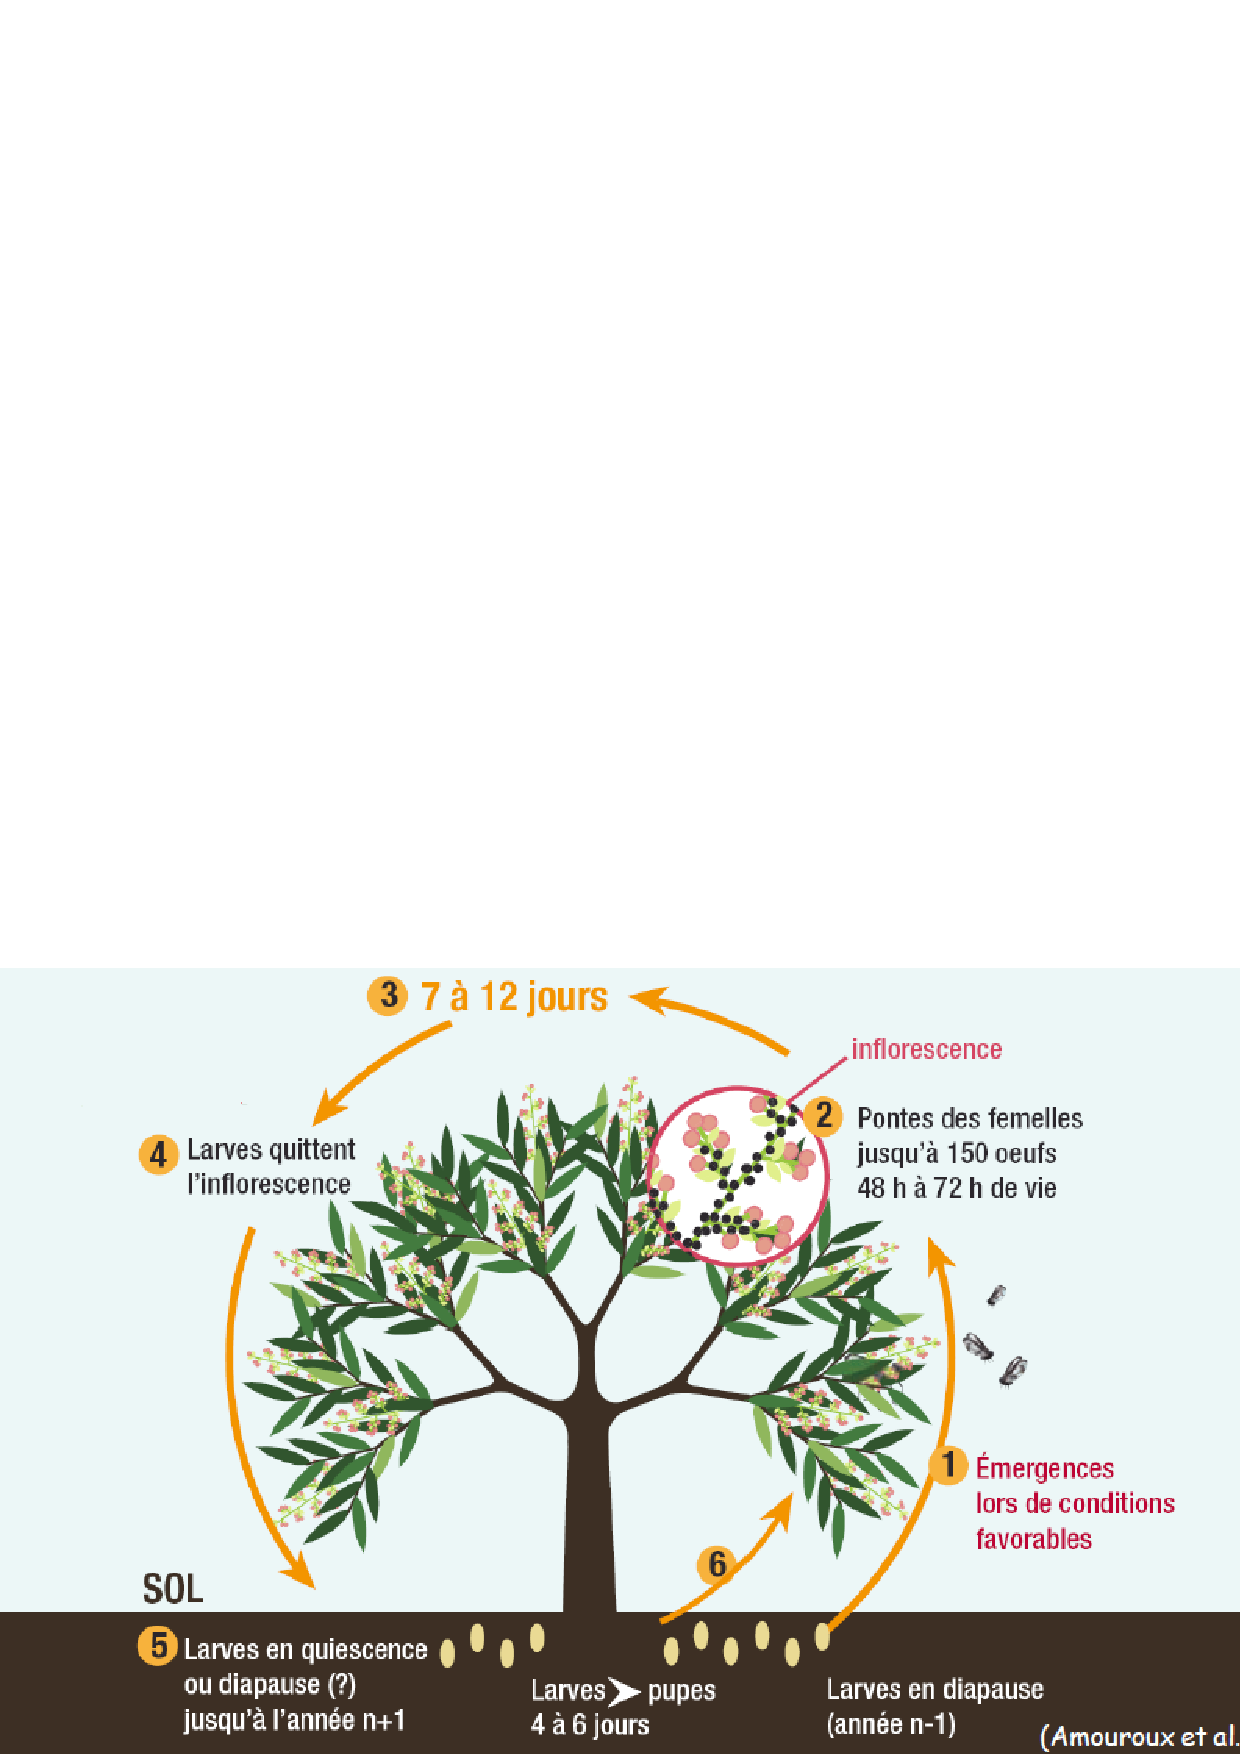
\includegraphics[scale = 0.33]{photos/cycle.png}
%  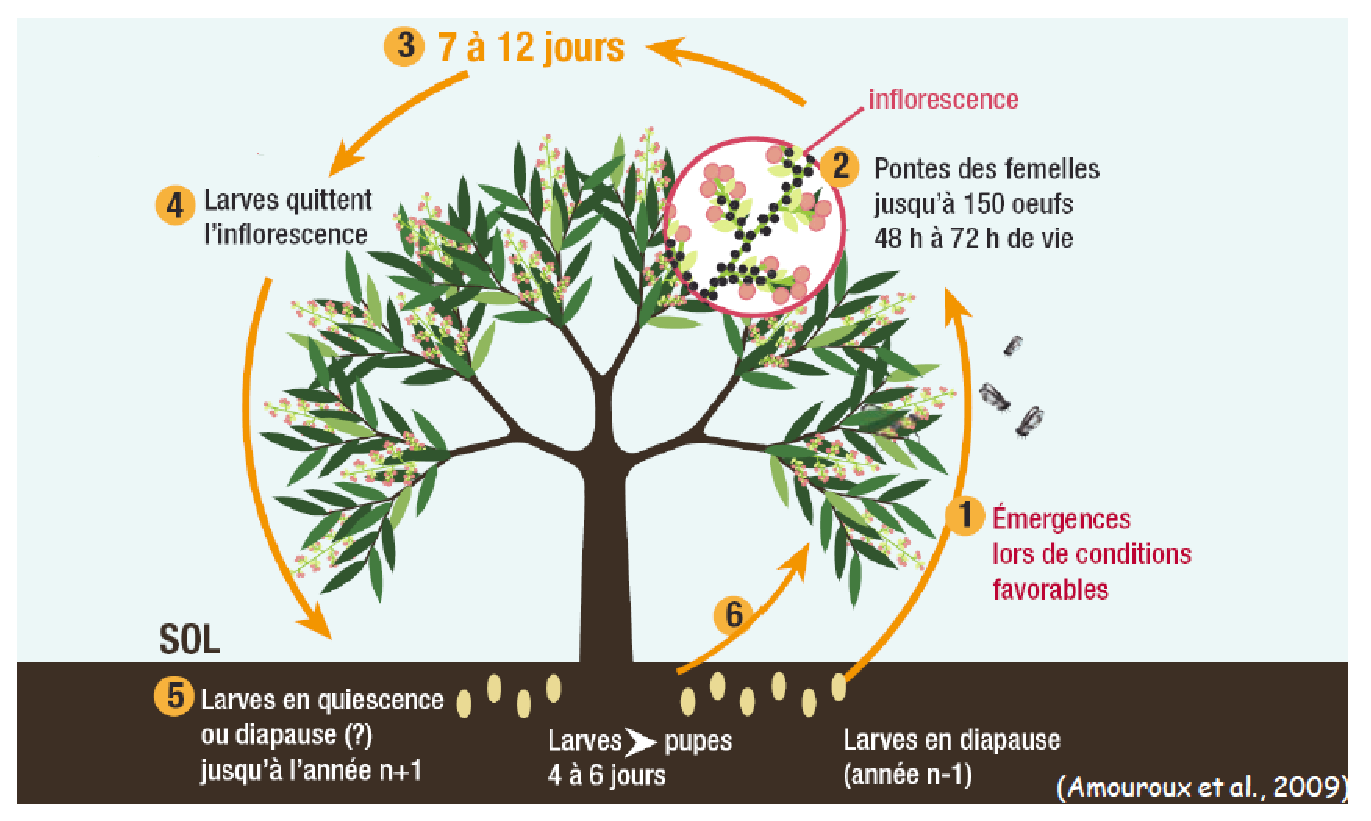
\epsfig{file = photos/cycle.eps, scale = 0.5}
 \caption{Représentation du cycle de développement de la cécidomyie des fleurs du manguier par \citet{paulguide}.}
 \label{fig:cycle}
\end{figure}
%

% \subsection{Titre random}

Les individus qui sortent de diapause permettent notamment le lancement de la dynamique d'infestation pendant la période de floraison.
La sortie est dû à une baisse de température qui coïncide avec le début de la floraison \citep{pauldiap}.
























